\documentclass{EPL-master-thesis-covers-FR}

\title{HaïtiWater 2.0}
\subtitle{Evolution de l'application HaïtiWater vers une application entière  fonctionnelle hors-ligne}

\author{Vincent \textsc{Gradzielewski}}% Handcrafted third author :D

\degreetitle{Master [120] en sciences informatiques}

\supervisor{Kim \textsc{Mens}}
\secondsupervisor{Sandra \textsc{Soares-Frazão}}

\readerone{}
\readertwo{}

\years{2020-2021}

\usepackage{subcaption}
\captionsetup{compatibility=false}
\usepackage{hyperref}
\usepackage{cite}
\usepackage{float}
\usepackage{multirow}
\usepackage{multicol}
\usepackage[final]{pdfpages}
\usepackage{booktabs}
\usepackage{multirow}
\usepackage{graphicx}
%\usepackage[toc]{multitoc}
%Vérifier la table des matière (une colonne)

\usepackage{amssymb}% http://ctan.org/pkg/amssymb
\usepackage{pifont}% http://ctan.org/pkg/pifont
\newcommand{\cmark}{\ding{51}}% pour les checkmark
\newcommand{\xmark}{\ding{55}}%

\frenchbsetup{StandardLists=true} % Resolves conflict between babel and enumitem
\usepackage{enumitem} % better formating of lists

\usepackage[style=long,nonumberlist,toc,xindy,acronym,nomain]{glossaries}
%Vé
\makenoidxglossaries

\begin{document}

	\maketitle
	\tableofcontents

	\setlength{\parskip}{1.5em plus1em minus1em}

	% Total des pages : entre 49 et 75 d'après nos estimations.

	\chapter*{Résumé}
	\addcontentsline{toc}{chapter}{Résumé}
	
		%Objectif, solution, évaluation
	
		Ce travail de fin d'études a été réalisé dans le cadre de mon Master en Sciences Informatiques à l'École Polytechnique de Louvain-la-neuve durant l'année académique 2020-2021.
		
		Dans ce mémoire je vais présenter mon travail qui consistait à reprendre l'application HaïtiWater développée précedemment par Adrien Hallet, Céline Deknop et Sebastien Strebelle qui a pour but "La gestion du réseau de distribution d'eau potable en Haïti". Le but étant de faire évoluer cette application pour que celle-ci soie entièrement
		
		
		 afin de la faire évoluer vers une application web qui serait entièrement utilisable \textbf{hors-ligne}.
		 
		Cette application a pour but "La gestion du réseau de distribution d'eau potable en Haïti". Je commencerai par une brève introduction sur le contexte Haitien et sur les raisons pour lesquels l'évolution de cette application était nécessaire. Ensuite je présenterai le principe des progressive weba app et pourquoi j'ai choisis d'utiliser cette technologie plûtot qu'une autre. Je présenterai ensuite la validation de l'application et les feedbacks que j'ai reçu des utilisateurs ainsi que les conséquence de cette validation sur l'application finale. Puis je concluerai par une liste des améliorations possibles.

		Tout le travail réalisé est disponible ici :

\begin{itemize}
	\item Github : \url{https://github.com/exavince/HaitiWater}
	\item Par l'UCL : \url{https://haitiwater.sipr.ucl.ac.be}
	\item En Haïti : \url{unknown}
\end{itemize}		

		Si vous désirez tester l'application, il suffit de vous rendre sur un des liens cité précedemment et de vous connecter à l'aide de l'uilisateur qui vous sera communiqué si vous en faite la demande. Ces données ne seront pas révélées ici car les données ne peuvent pas être modifiéés aléatoirement. 
		

	\chapter*{Remerciements}
	\addcontentsline{toc}{chapter}{Remerciements}

		

	%\printnoidxglossary[title=Glossaire, toctitle=Glossaire]
	%\glsaddall

	\chapter{Introduction}

		
		\subsection*{Contexte}
		
			Ce mémoire appartient à un projet de développement financé par ARES-CCD avec quelques partenaires tels que Protos\footnote{\href{https://www.protos.ngo/fr/}{www.protos.ngo}}, l'UCL et l'UEH. 
			
			protos est une ONG qui vise à améliorer l'accès à l'eau potable dans plusieurs pays du monde afin de les aider à se développer. 
			
			Suite à de nombreuses crises politiques et catastrophes naturelles qui ont détruit beaucoup d'infrastructures locales, l'accès à l'eau potables est devenu difficile en Haïti. De plus, des incertitudes politiques entravent la reconstruction de ces installations et les populations ne sont pas toujours aidées par les services publics pour assurer la distribution de l'eau. 
			
			Il y a quelques années Protos est entré en contact avec l'UCL afin de réaliser un système logiciel pilote pour la gestion de la distribution d'eau potable en zone rurale. C'est pour cette raison que l'ONG Protos est active dans le pays depuis quelques années et à permis aux anciens mémorants de créer l'application HaïtiWater.
			
			 En effet, aucune gestion centralisée organisée par l'Etat n'existe pour ces zones, éloignées des grandes agglomérations. Des réseaux existent, constitués de points de prélèvement d'eau, de conduites de distribution d'eau et de fontaines situées dans les villages, mais la gestion publique de ceux-ci n'est pas opérationnelle. 

			L'application créée précedemment propose un appui à ces organismes locaux afin de mieux organiser cette distribution. 
			%Explication de l'application des différents modules existants

			

		\subsection*{Problématiques}
		
			Actuellement l'application HaïtiWater est prévue pour fonctionner uniquement lorsque le réseau est stable et fonctionnel. Malheureusement en Haïti le réseau est assez instable et par endroit ce réseau n'est même pas disponible. La suite du développement de l'application va donc devoir porter sur le fonctionnement hors-ligne de celle-ci. 

			% Expliquer pourquoi l'application a besoin d'évoluer 

		\subsection*{Motivation}

			%Explqiuer pourquoi avoir choisis ce mémoire
			

		\subsection*{Objectifs}

			%Expliquer le but final du mémoire au niveau de l'usage de l'applcition en Haiti
			
		\subsection*{Approche}

			%Expliquer les différentes étapes par lesquelles je suis passé pour réaliser ce mémoire (étude des différentes tech, développement, validation, ...)
			
		\subsection*{Contribution}

			%Qu'est ce qu'a apporté le travail réalisé
			%Qu'elle est la plus value ?

		\subsection*{Plan}

			%Explication dans le temps des différentes phases de travail 

	\chapter{Contexte}


		\section{La gestion de l'eau en Haïti}
			\label{sec:situation}
			
				Haïti est l'un des pays les plus pauvres au monde. Le pays est situé dans une zone géographique où les risques de catastrophes naturelles sont très éleves. Ces intempéries détruisent les infrastructures et empêchent le bon développement des réseaux de distribution d'eau. Il y a quelques années, en 2010, le pays a subit un énorme séisme qui a ravagé une bonne partie du territoire. Parmi tous les défis à relever vient celui de la gestion et de la distribution de l'eau potable sur le territoire, surtout dans les zones les plus rurales. Le climat de la région rendant excessivement difficle l'exploitation directe des cours d'eau, il faut beaucoup d'infrastructures afin de pouvoir asssumer la distribution de l'eau potable à tous.
				
				En raison de la grande pauvreté et de gros problèmes organisationnels qui règnent sur la plupart de l'île, il est très difficile de maintenir et de développer le réseau de distribution d'eau potable. Il y a un gros manque de collaboration entre les entités haïtiennes ou entre les villages dû en partie à la communication qui n'est pas du tout optimmisée voir inexistante dans certains cas. Dans les zones les plus rurales de l'île, le taux de recouvrement des factures est excessivement faible, jusqu'à 11\%.
				
				Pour toutes ces raisons, l'ONG Protos vient donc en aide à Haïti afin d'aider le service national des eaux à gérer la gestion des infrastructures et la facturation des clients surtout dans les zones rurales.
				
				Si vous désirez plus d'informations sur les problèmes environementaux, politiques, sociaux ou organisationnels du contexte haïtiens, je vous invite à aller consulter le mémoire d'Adrien Hallet, Céline Deknop et Sébastien Strebelle \cite{ref:haitiwater}.

				%Brève explication sur le contexte Haïtien


		\section{Introduction à l'application}
				Dans le cadre de la situation décrite dans la section \ref{sec:situation} (La gestion de l'eau en Haïti), Protos a fait appel à l'UCL afin de créer une application d'aide à la gestion et la distribution de l'eau potable en Haïti. Une première version de l'application a été développée en 2018-2019 par 3 personnes dans le cadre de leur mémoire \cite{ref:haitiwater}, elle comprend différents modules permettant de faciliter la gestion des infrastuctures et les clients qui vont y chercher de l'eau.
				
				L'application est basée sur un principe hiérarchique. Pour illustrer celle-ci je vais reprendre l'image présentée ici \cite{ref:haitiwater}. 
				
				\begin{figure}[H]
					\centering
					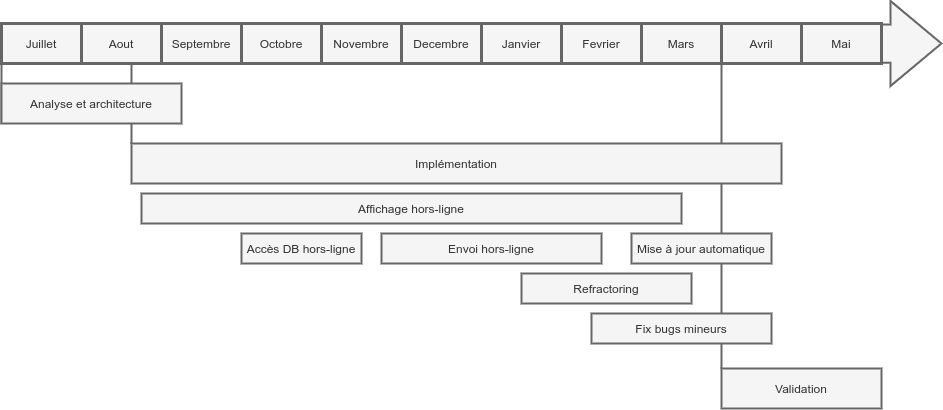
\includegraphics[width=0.5\textwidth]{images/Gantt}
					\caption{Module consommateurs}
				\end{figure}
				
				
			\subsection{Eléments de l'application}
				\begin{description}
					\item[Zone] Une zone représente une partie du territoire. Une zone peut être subdivisée en plusieurs sous-zone, la zone-parent reprendra alors toutes les donées des zones enfants. Cela permet de séparé les responsablités des différents territoires.
					\item[Element du réseau] Ces éléments représent les points physiques du réseau de distribution d'eau potable. Ces éléments sont au nombre de 6 : conduites, réservoirs, sources, fontaines, kiosques et prises individuelles. Tous ensembles ils forment le réseau de distribution au complet. 
					\item[Consommateurs] Le consommateur est une personne qui va utiliser le réseau de distribution d'eau potable. Chaque consommateur se voit lors de son enregistrement attribué à un seul élément de sortie d'eau du réseau : fontaine, kiosque, prise individuelle. De cette façon, il est plus simple de gérer la facturation des consommateurs.
				\end{description}
				
			
				
				%Inclusion du schéma zones, fontaines, ... pour rendre la suite plus claire.
				
			\subsection{Utilisateurs de l'application}
				Il y 2 types d'utilisateurs qui peuvent se connecter à l'application
				
				\begin{description}
					\item[Gestionnaire de fontaine] Ce gestionnaire va gérer la distribution de l'eau aux différents consommateurs. Il devra gérer tous les éléments du réseau qui lui sont attribués.
					\item[Gestionnaire de zone] Ce gestionnaire va avoir la responsabilité de gérer d'autres gestionnaires de zones et/ou des gestionnaires de fontaines. Sont travail est plus d'administrer et de surveiller les personnes qui sont en dessus de lui.			 
				\end{description}
				
				Ces deux gestionnaires vont avoir des privilèges différents et peuvent donc intéragir différemment sur les données. Pour illustrer plus simplement cela, voici un tableau tel que présenté ici \cite{ref:haitiwater} où vous pourrez retrouver plus d'informations sur les rôles des différents gestionnaire. 
				\begin{table}[H]
					\centering
					\small
					\setlength\tabcolsep{2pt}
					\begin{tabular}{|l|c|c|}
						\hline
						\multirow{2}{*}{\textbf{Permission}} & \multicolumn{2}{l|}{\textbf{Gestionnaire de}} \\ \cline{2-3}
						 & \textbf{fontaine} & \textbf{zone} \\ \hline
						 Ajouter/modifier/supprimer un consommateur & \cmark & \cmark \\ \hline
						 Ajouter/modifier/supprimer un élément du réseau de distribution & \cmark & \cmark \\ \hline
						 Ajouter/modifier/supprimer un rapport mensuel & \cmark & \cmark \\ \hline
						 Ajouter/modifier/supprimer un paiement & \cmark & \cmark \\ \hline
						 Ajouter/modifier/supprimer un ticket de support & \cmark & \cmark \\ \hline
						 Ajouter/modifier/supprimer une zone & \xmark & \cmark \\ \hline
						 Ajouter/modifier/supprimer un gestionnaire & \xmark & \cmark$^{*}$ \\ \hline
						 Accepter/refuser un changement dans l'historique & \xmark & \cmark \\ \hline
						 \multicolumn{3}{p{\textwidth}}{\emph{* : Un gestionnaire de zone ne peut pas modifier les informations personnelles (mot de passe, courriel, nom, prénom) d'un gestionnaire existant}} \\
					\end{tabular}
					\caption{Permissions dans l'application, par type d'utilisateur}
					\label{tab:permissions}
				\end{table}
				
			\subsection{Accueil}
				Ce module contient les informations condensées de la zone qui est attribuée à l'utilisateur. Il peut y retrouver le nombre de fontaines, de kiosques, de points de prises individuelles et de conduites que contient sa zone mais aussi le nombre de foyers et de consommateurs individuels liés à celle-ci. 
								
				\begin{figure}[H]
					\centering
					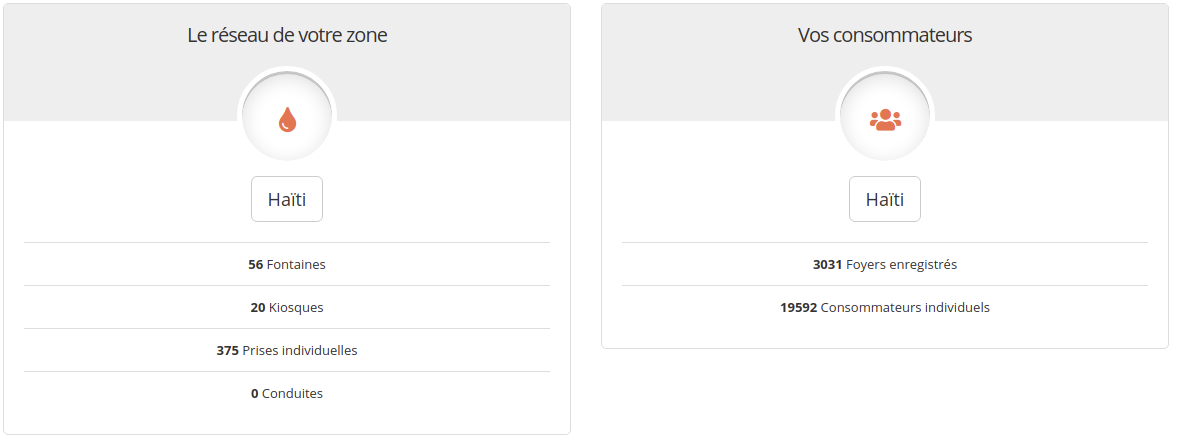
\includegraphics[width=1\textwidth]{images/dashboard}
					\caption{Module d'accueil}
				\end{figure}
				
				
			\subsection{Réseau}
				\label{sec:reseau}
				Dans ce module, l'utilisateur peut retrouver 3 éléments différents.
				
				\begin{description}
				\item[Schéma] Un schéma contenant la répartition des consommateurs par genre ou le volume d'eau mensuel distribué dans chaque zone. Il peut sélectionner le schéma à afficher grâce à une liste déroulante.
				\item[Résumé de zone] Un résumé de sa zone géographique contenant le nombre de consommateurs et de points d'eau présents ainsi que le volume d'eau distribué dans celle-ci.
				\item[Elements du réseau] Un tableau interactif qui contient tous les différents éléments du réseau. Dans cette partie en fonction de ses privilèges, celui-ci peut supprimer, modifier ou ajouter des éléments du réseau. Il peut également trier ou faire des recherche dans ce tableau selon ses besoins.
				\end{description}
				
				\begin{figure}[H]
					\centering
					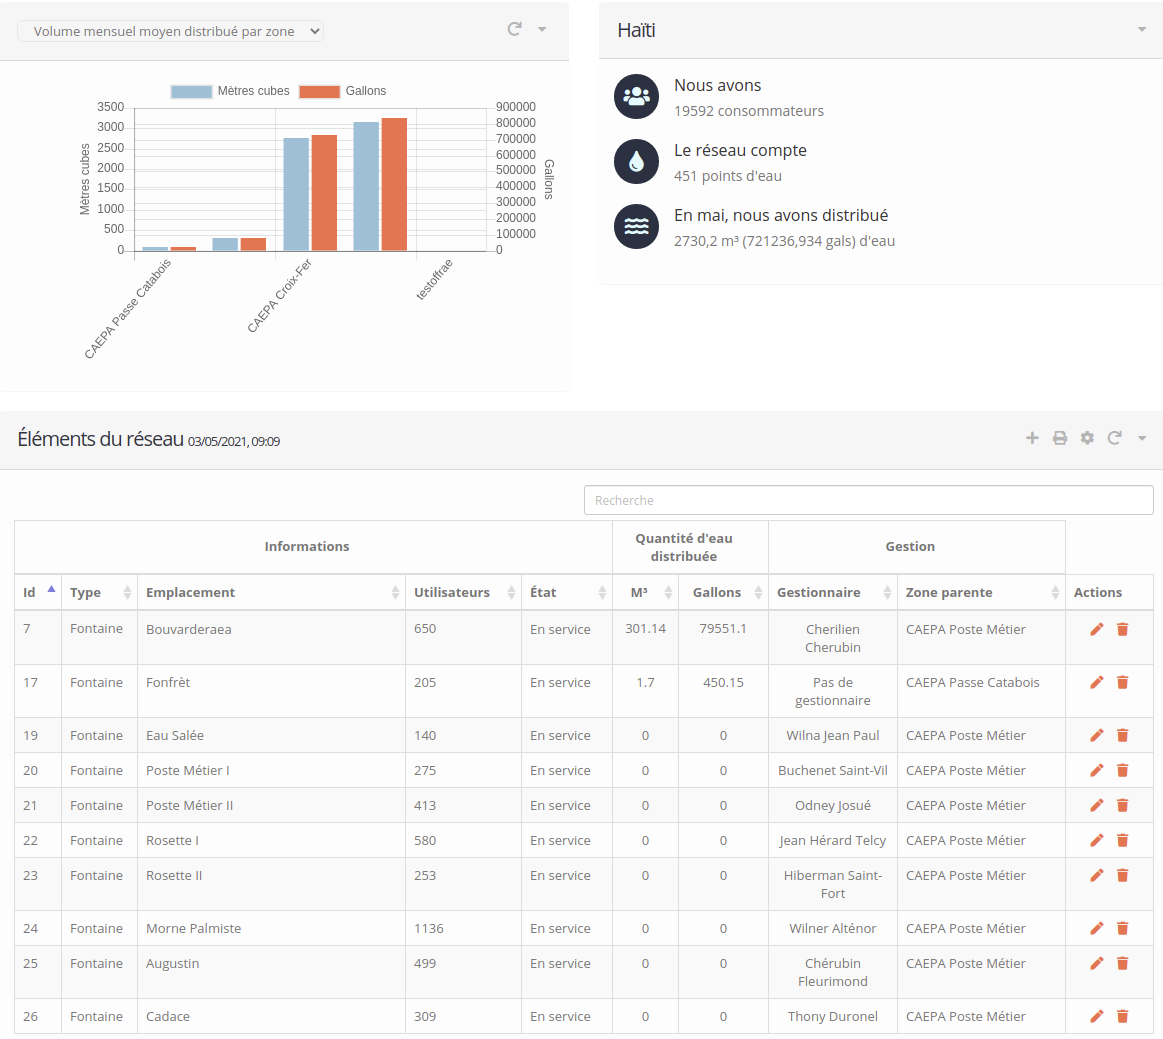
\includegraphics[width=1\textwidth]{images/water_elem}
					\caption{Module réseau}
				\end{figure}
				
\newpage
				
			\subsection{Carte}
				Ce module comprend un tableau réduit des éléments du réseau ainsi qu'une carte interactive qui permet à l'utilisateur de voir où sont situés les différents éléments du réseau et de connaître ou d'encoder les coordonnées géographiques de ceux-ci. 
				
				Comme dans le module \ref{sec:reseau} "Réseau", il est également possible d'ajouter, modifier ou supprimer des éléments du réseau. De plus c'est ici que l'on peut ajouter des coordonnées géograpqiues à un élément du réseau. Soit en les entrants manuellements soit en utilisant la carte interactive.
				\begin{figure}[H]
					\centering
					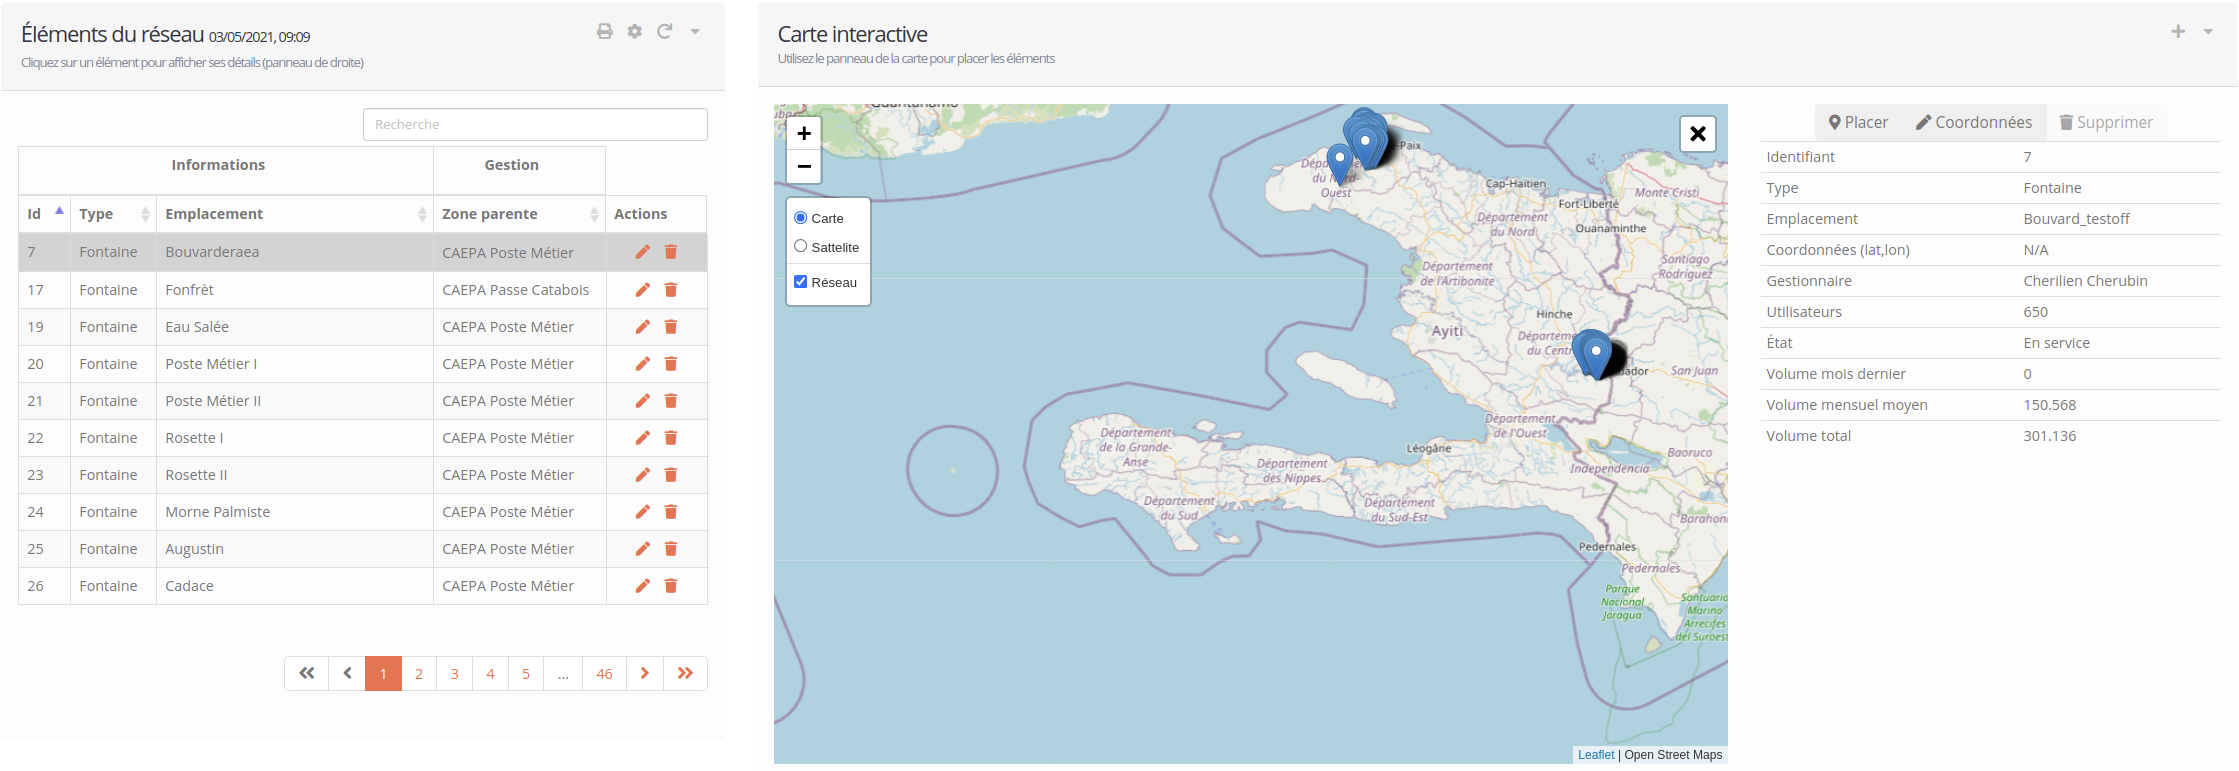
\includegraphics[width=1\textwidth]{images/map}
					\caption{Mordule carte}
				\end{figure}
				
				\begin{figure}[H]
					\begin{subfigure}[b]{0.5\textwidth}
  						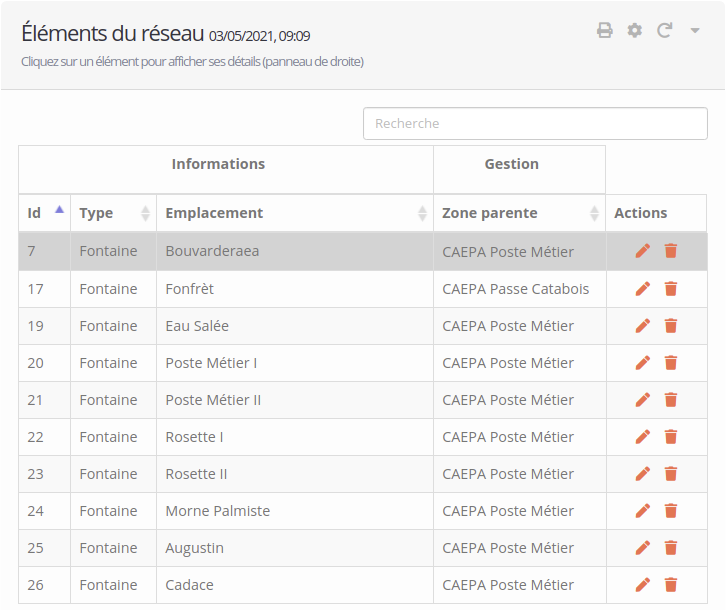
\includegraphics[width=1\linewidth]{images/map_tab1}
  						\caption{Tableau des éléments réseaux simplifié}
					\end{subfigure}%
					\begin{subfigure}[b]{0.5\textwidth}
  						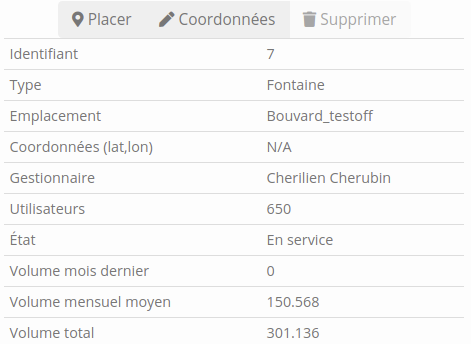
\includegraphics[width=1\linewidth]{images/map_tab2}
  						\caption{Détails de l'élément réseau}
					\end{subfigure}
					\label{fig:test}
				\end{figure}
				
			\subsection{Gestion de zone}
				Ce module comprend 3 tableaux permettant à l'utilisateur de gérer sa zone.
				\begin{description}
					\item[Zones] Le premier contient les différentes zones géographiques encodées dans le système. Cliquer sur un des éléments du tableau permet de filtrer les éléments des deux autres tableaux qui seront décrits plus bas afin de ne garder que les éléments de la zone concernée. Ce tableau permet également si l'utilisateur a les privilèges requis d'ajouter, supprimer ou modifier une zone.
					\item[Gestionnaires] Le deuxième contient la liste de tous les gestionnaires. Cliquer sur un gestionnaire permet à l'utilisateur de filtrer les éléments réseaux qui sont gérés par ce gestionnnaire. De nouveau si l'utilisateur possède les privilèges nécessaires, il pourra ajouter, modifier ou supprimer des gestionnaires.
					\item [Elements du réseau] Le dernier contient le même tableau que dans la section \ref{sec:reseau} "Réseau".
				\end{description}
				\begin{figure}[H]
					\centering
					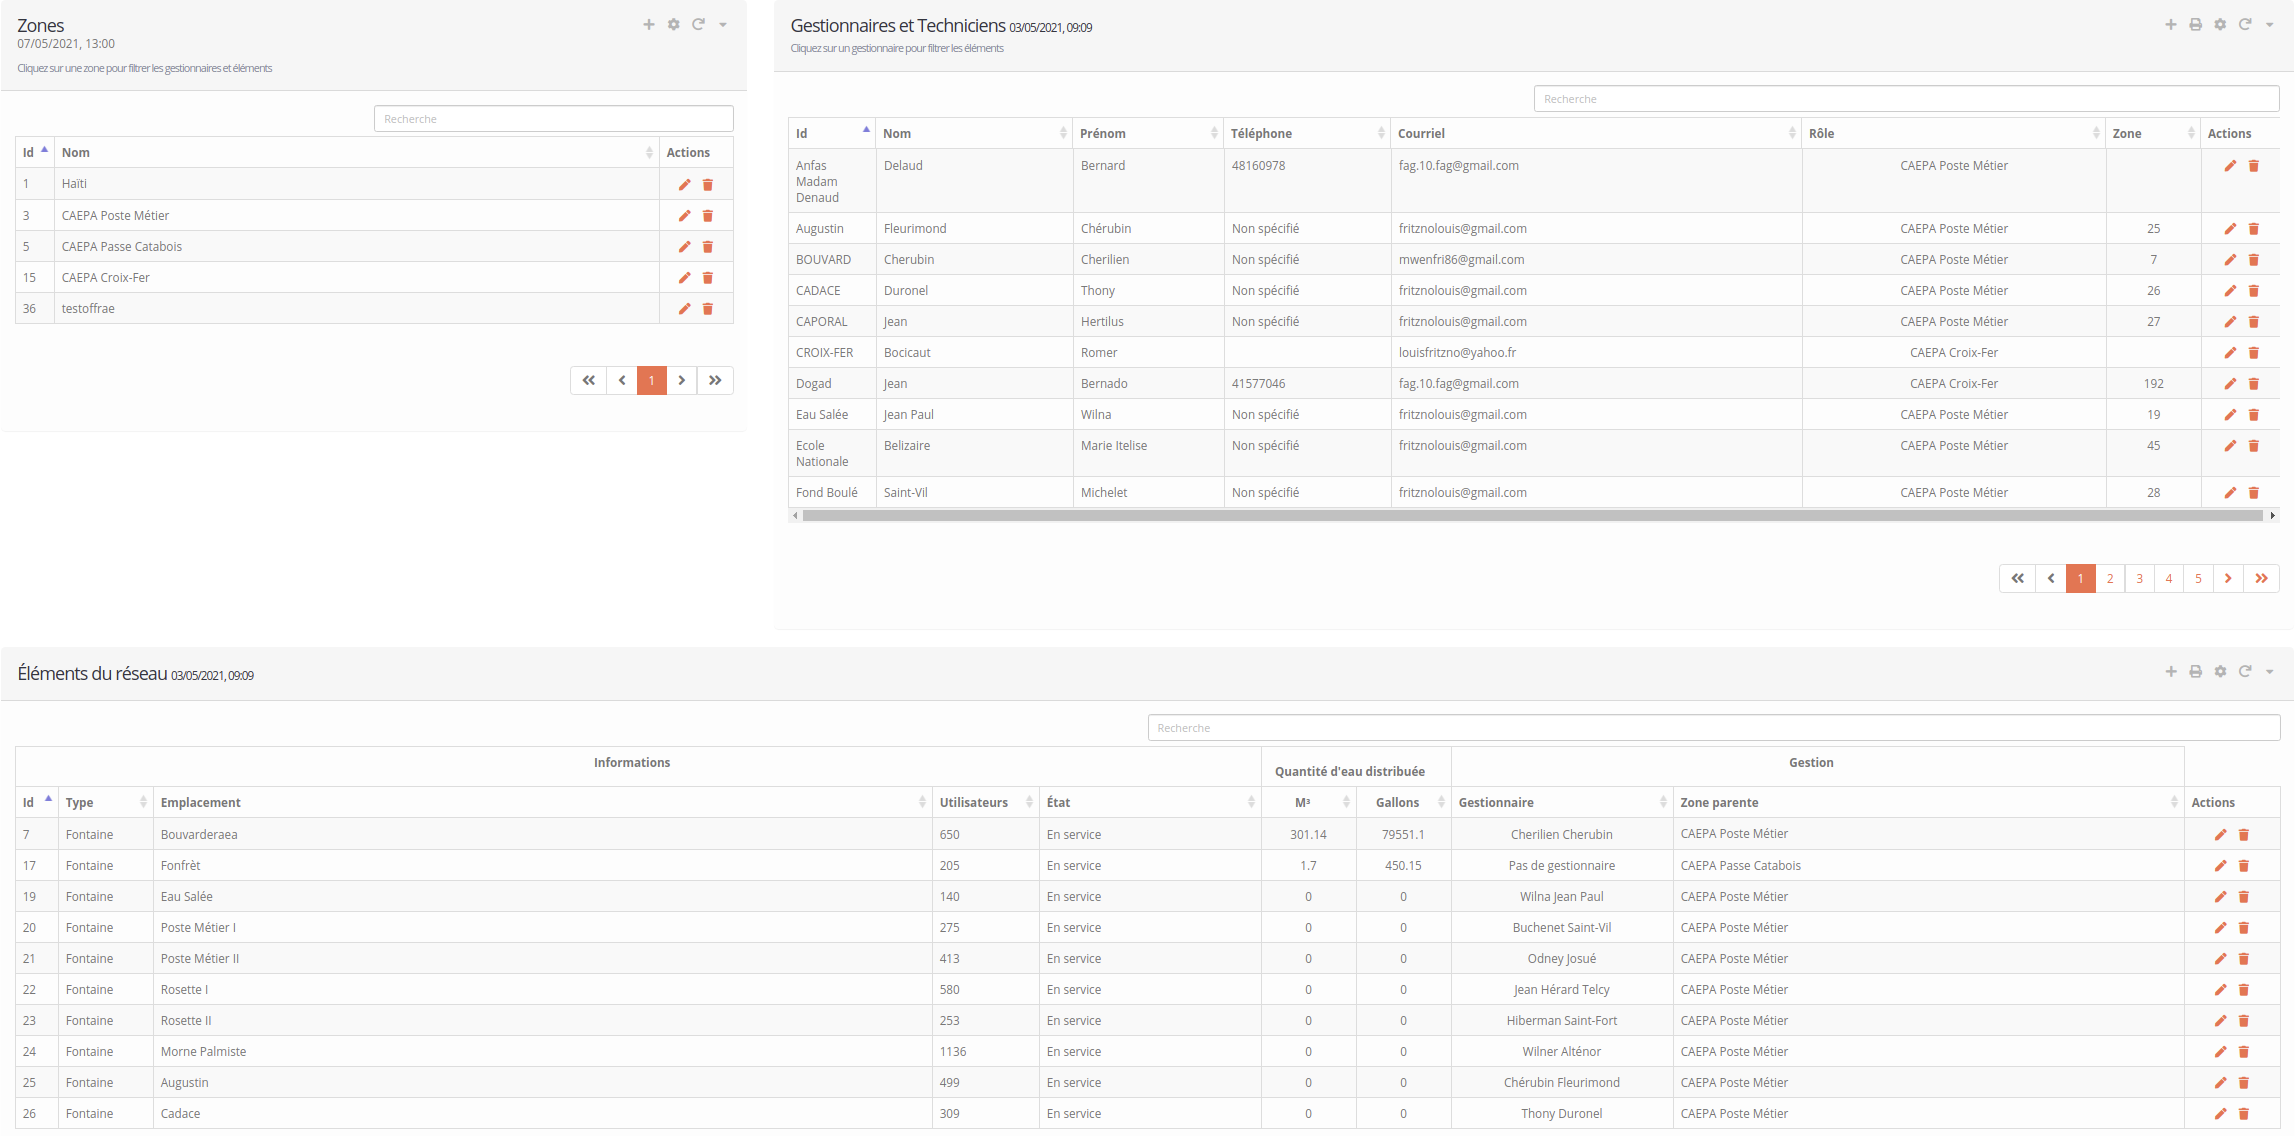
\includegraphics[width=1\textwidth]{images/gestion}
					\caption{Module gestion de zone}
				\end{figure}
			
				
				\begin{figure}[H]
					\begin{subfigure}[b]{0.3\textwidth}
  						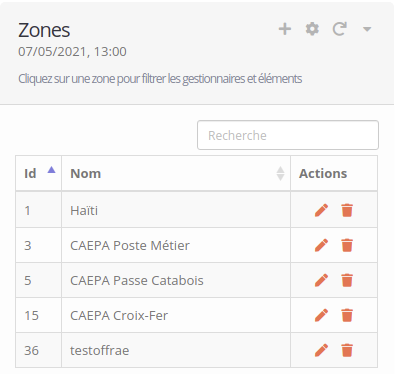
\includegraphics[width=1\linewidth]{images/gestion_tab1}
  						\caption{Tableau des zones}
					\end{subfigure}%
					\begin{subfigure}[b]{0.7\textwidth}
  						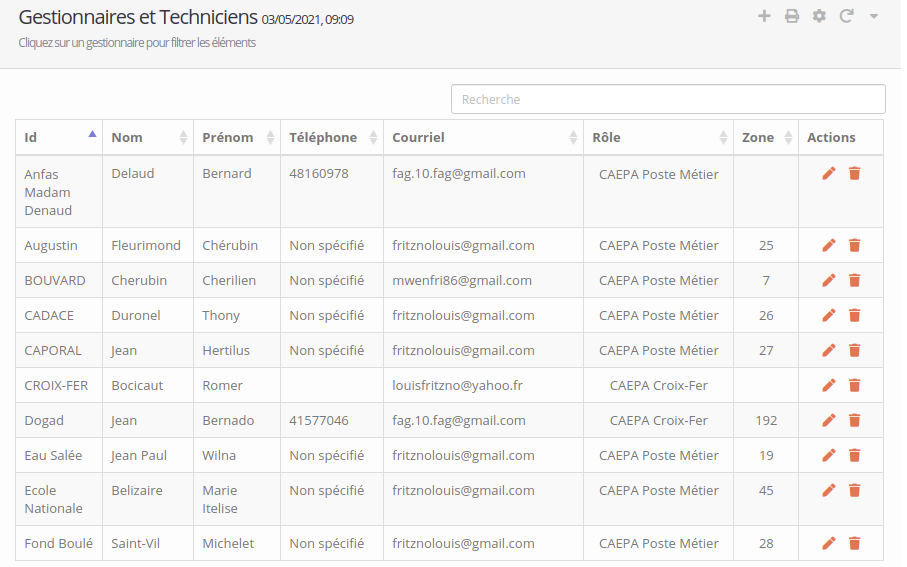
\includegraphics[width=1\linewidth]{images/gestion_tab2}
  						\caption{Tableau des gestionnaires}
					\end{subfigure}
					\label{fig:test}
				\end{figure}
			
			\subsection{Historique}
				Ce module contient les actions ayant été effectuées par des gestionnaires de fontaines. Ces actions doivent être validées ou refusées par un gestionnaire plus haut placé. On peut y retrouver deux tableaux.
				\begin{description}
					\item[A valider] Le tableau du haut contient les éléments devant être validés. Ici si l'utilisateur a les privilèges requis, il peut choisir de confirmer ou non un action qui a été encodée.
					\item[Historique] Le tableau du bas contient les éléments qui ont été validés ou refusés dans les 3 dernières semaines. Il s'agit simplement d'un historique récent.
				\end{description}
				\begin{figure}[H]
					\centering
					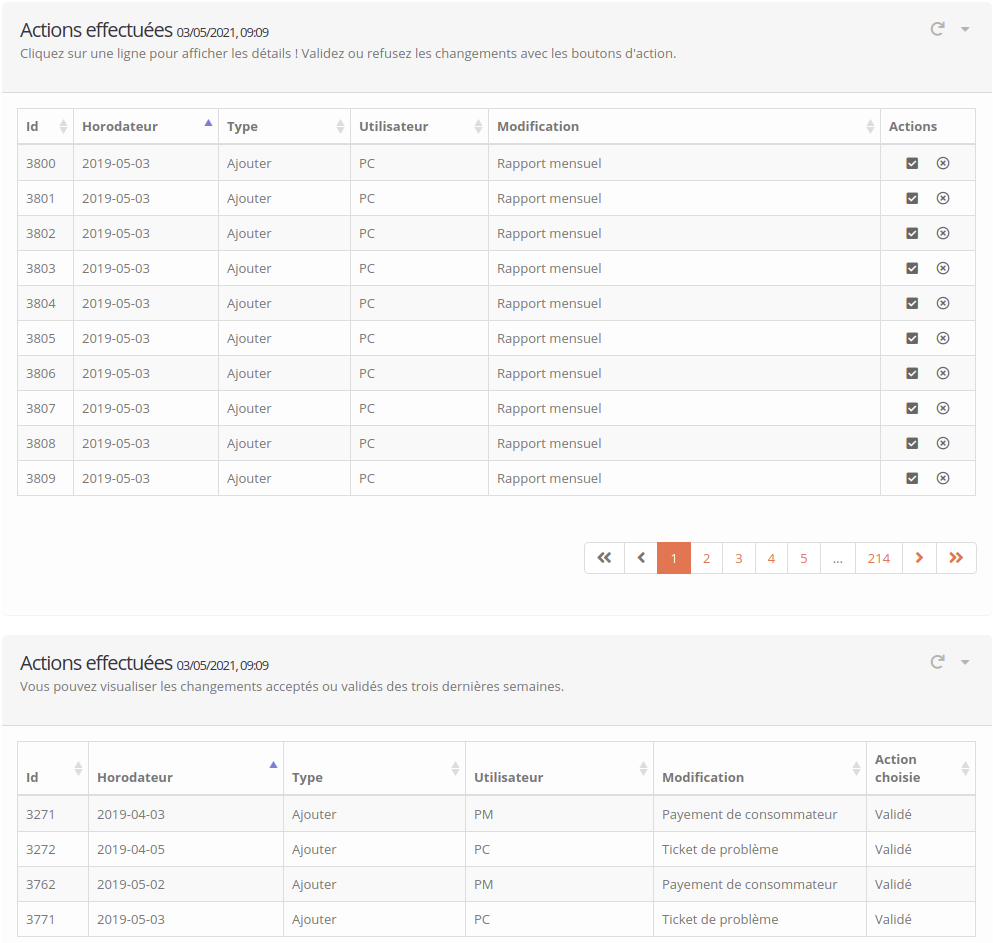
\includegraphics[width=1\textwidth]{images/logs}
					\caption{Module historique}
				\end{figure}
			
			\subsection{Rapports}
				Dans ce module, l'utilisateur peut signaler les différents problèmes qu'il rencontre avec les infrastructures de distribution d'eau. Une fois le problème signaler, celui-ci peut consulter ce qu'il a encodé dans le tableau juste en dessous et modifier ou supprimer son signalement. Si ses privilèges sont suffisament élevés, il pourra également gérer les signalements des autres personnes.
				
				C'est également ici que l'utilisateur va pouvoir encoder les rapports mensuels. Si jamais la connexion internet n'est plus présente, il pout simplement enregistrer le formulaire avec les données qu'il a encodée afin de l'envoyer plus tard lorsque le réseau sera de nouveau accessible.
				
				\begin{figure}[H]
					\centering
					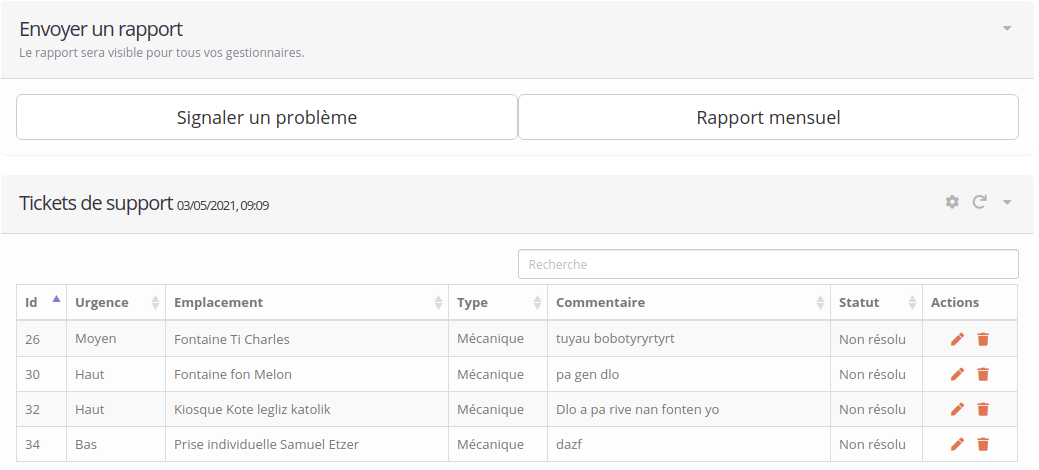
\includegraphics[width=1\textwidth]{images/report}
					\caption{Module rapport}
				\end{figure}
			
			\subsection{Consommateurs}
				Dans ce module, l'utilisateur retrouve 3 parties différentes :
				\begin{description}
					\item[Schéma] Le même choix de schéma que décris dans la section \ref{sec:reseau}.
					\item[Résumé de zone] Un résumé de la situation de votre zone (nombre de foyers consommant de l'eau, nombre de consommateurs, nombre de foyers n'ayant pas payé leur facture).
					\item[Consommateurs] Un tableau qui reprend tous les consommateurs auxquels l'utilisateur a accès. Celui-ci peut ajouter, modifier ou supprimer des consommateurs. Ou bien il peut également juste consulter tous les détails sur ceux-ci.
				\end{description}

				
				\begin{figure}[H]
					\centering
					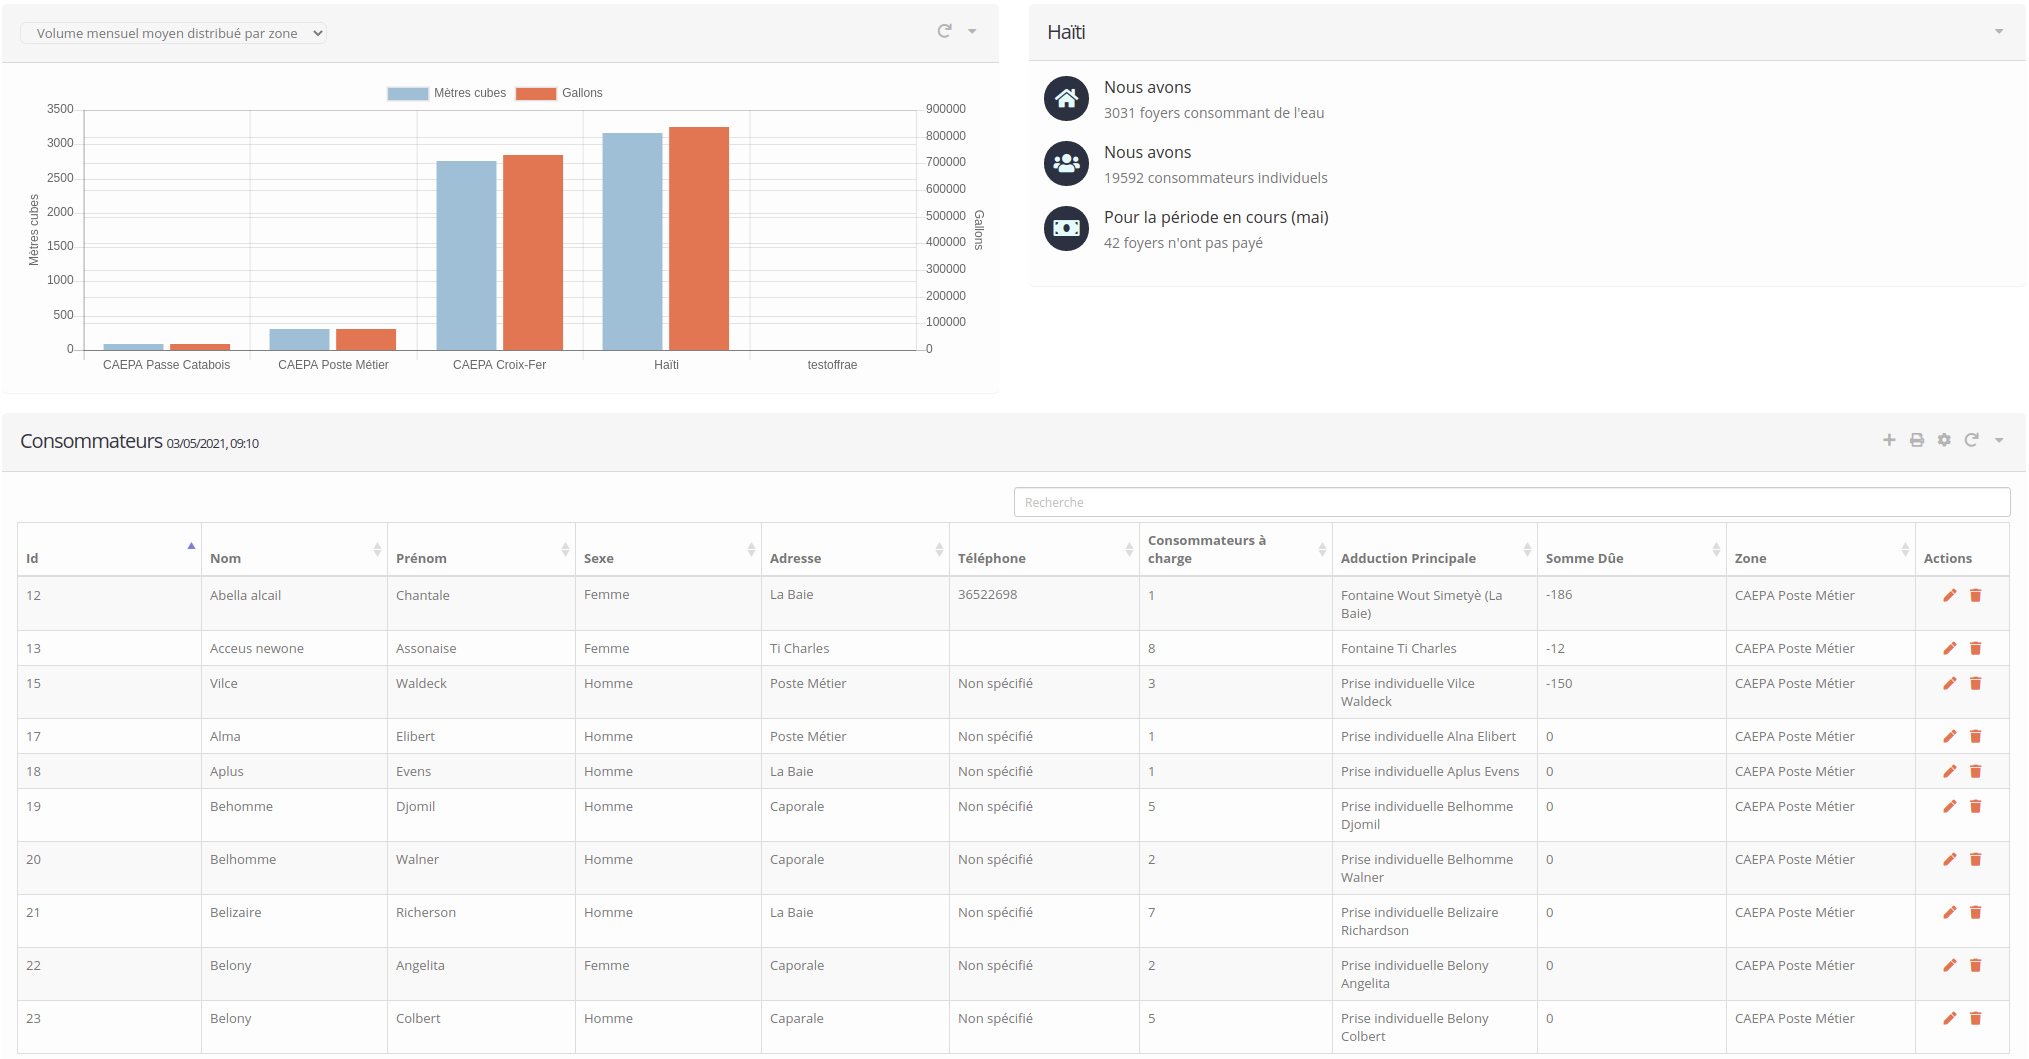
\includegraphics[width=1\textwidth]{images/consumer}
					\caption{Module consommateurs}
				\end{figure}
				
				\begin{figure}[H]
					\centering
					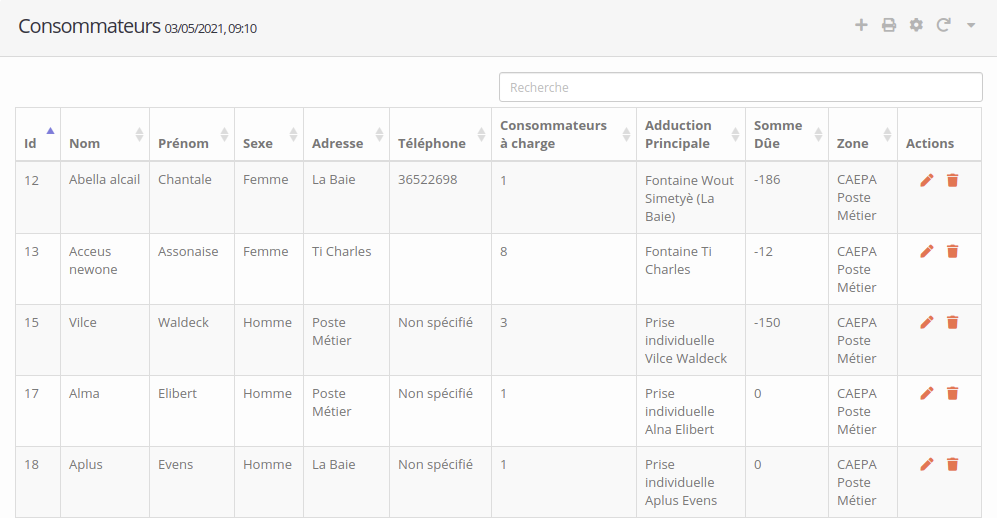
\includegraphics[width=1\textwidth]{images/consumer_tab1}
					\caption{Module consommateurs}
				\end{figure}
			
\newpage
			\subsection{Finances}
				Dans ce module, l'utilisateur a accès à 4 tableaux différents qui lui permettent de gérer les finances de ses consommateurs. Celui-ci pourra modifier, supprimer ou ajouter des informations dans les différents tableaux en foncion de son niveau de privilèges.
				\begin{description}
					\item[Zones] Un tableau contenant les différentes zones. Le fait de sélectioner une zone permet à l'utilisateur de filtrer les consommateurs en fonction de leur zone d'attribution.
					\item[Consommateurs] Un tableau contenant les consommateurs auxquels l'utilisateur a accès. Le fait de sélectionner un consommateur permet de faire apparaître les deux tableaux suivants.
					\item[Détails] Un tableau contenant les coordonnées du consommateur sélectionné ainsi que la somme dûe par celui-ci. Il n'est pas possible de modifier des données manuellements dans ce tableau.
					\item[Paiements] Un tableau interactif contenant tous les paiements effectués par le consommateur sélectionné. Ici l'utilisateur peut ajouter, modifier ou supprimer des paiements.
				\end{description}
				
				\begin{figure}[H]
					\centering
					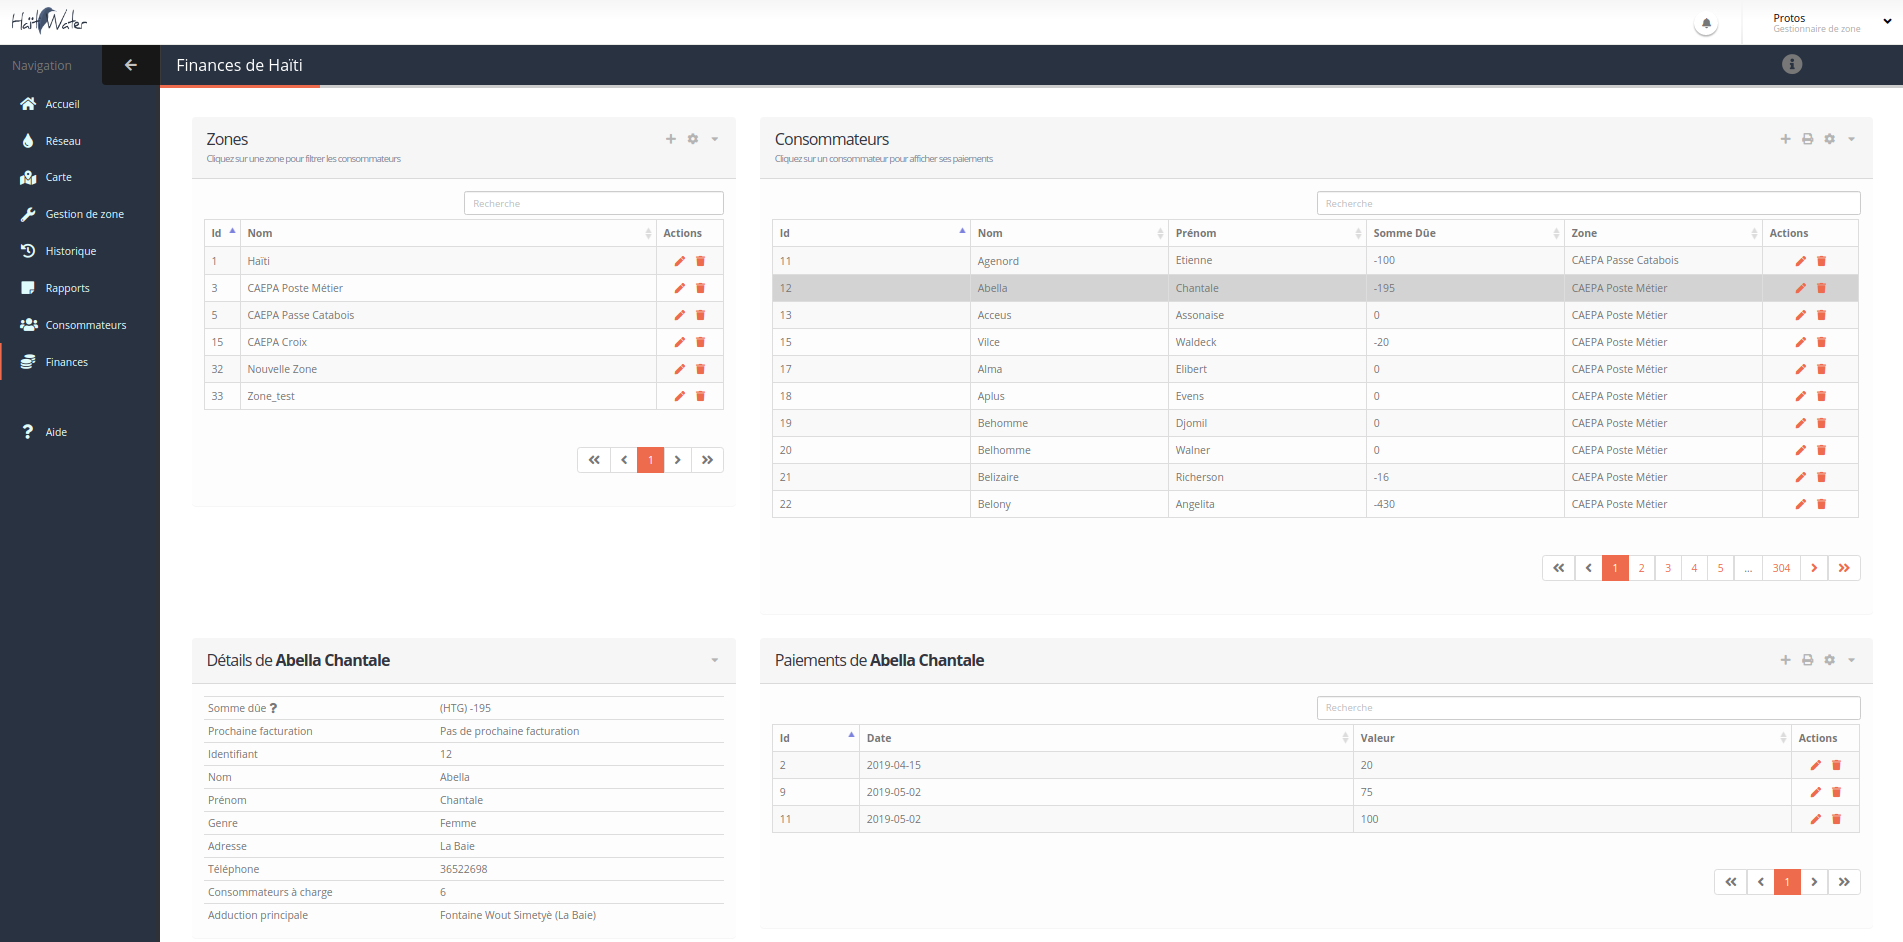
\includegraphics[width=1\textwidth]{images/finances}
					\caption{Module finances}
				\end{figure}
				
				
		\section{Problèmes réseaux}
			L'application HaïtiWater est une application web classique. Cela signifie que pour fonctionner, il faut qu'il y ait nécessairement une connexion à internet. Hors en Haïti, cette connexion n'est pas très stable en ville et celui-ci peut aller jusqu'à être inexistant lorsque vous vous aventurez dans les zones les plus rurales. 
			
			Ces problèmes de connexions font que l'application est difficilement utilisable sur le terrain en toute sérénité car on ne sait jamais quand le réseau va devenir capricieux. Pour pallier ce problème, il a été décidé de transformer l'application web existante pour que celle-ci puisse fonctionner même lorsque le réseau est absent.
				
			De part sa nature, une application web nécessite un connexion pour pouvoir fonctionner. Il a donc fallu étudier les différentes options qui pourraient permettre de faire fonctionner l'application hors-ligne. Parmis les ces options,  les deux qui ont été retenues étaient de soit créer une \textbf{application mobile} séparée de l'application web, soit de transformer l'application web existante en \textbf{Progressive Web App}. 
				
			L'avantage de créer une application dédiée aux mobiles est qu'il est très simple de gérer le fonctionnement hors-ligne de cette application. De plus on peut plus facilement utiliser les différentes capacités de l'appareil mobile comme la caméra, la localisation, ...
			L'inconvénient de cette solution est qu'il fallait du coup générer une nouvelle application de A à Z. De plus cela implique qu'il y aura deux codes différents dans deux langages différents à devoir maintenir.
				
			L'avantage de la Progressive Web App est que tout se joue au niveau du navigateur. Il n'est donc pas nécessaire de devoir maintenir un deuxième code source. De plus aucune installation n'est nécessaire de la part de l'utilisateur et les mises à jour de l'application sont faites de manière transparante.
			L'inconvénient de cette solution est que la gestion du mode hors-ligne est un peu plus complexe, on ne peut pas profiter des capacités de l'appareil mobile aussi bien qu'avec une application native et cette technologie étant assez récente, il n'y a pas énormément de ressource d'aide en ligne et tous les navigateurs ne prennent pas en charge toutes les fonctionnalités proposées.
				
			Au vu de la situation compliquée en Haïti et du temps qui sera alloué à ce mémoire, il a été décidé que la meilleure option était celle de la Progressive Web App. La raison principale est qu'il aurait difficile une fois le mémoire terminé d'avoir deux codes sources différents à maintenir et à mettre à jour.

	\chapter{Organisation}
		

		Etant le seul étudiant à réaliser ce mémoire, il n'a pas été nécessaire d'utiliser des outils de plannification complets. Cette section contiendra surtout la plannification des différentes tâches à accomplir permettant l'aboutissement de l'application ainsi que l'écriture de ce mémoire. Celles-ci ont été mises place grâce aux discussions avec mes deux promoteurs et une étudiante en informatique venue d'Haïti pour en apprendre plus sur l'application. 

		\section{Approche de travail}
			Comprendre les enjeux et les différentes problématiques a été la première tâche à accomplir. Il a fallut décider du type de technologie à utiliser afin d'apporter les fonctionnalités nécessaires au bon fonctionnement de l'application. 
			
			La meilleure option aurait été de pouvoir en discuter avec la plupart des acteurs en Haïti afin d'avoir le plus d'avis possible sur la question. Mais vu le temps que cela aurait pris cette option n'était pas du tout envisageable. Pour pallier à se problème, nous avons étudié la question avec mes deux promoteurs et Nahomie l'étudiante venue d'Haïti. Celle-ci à pu nous apporter son expertise afin de choisir l'option idéale.
			
			Une fois le choix technologique fait, nous avons effectuer la plannification des tâches.
		
		

			%Etude du problème
			%Prioritisation des taches

			\subsection*{Planification}
				\label{sec:planification}
				
				\paragraph*{Mensuel}
				Dans un premier temps, il a fallu réaliser un plan général de déroulement du mémoire. il a fallu mettre en avant les modules sur lesquels il fallait travailler en priorité et les différentes fonctionnalités à implémenter dans ceux-ci.   Nous avons essayer de déterminer certaine deadline afin de garantir la continuité de l'avancement du projet. Malgrès il était difficile de mettre des dates fixes car la technologie utilisée comporte encore peu de communauté et il est donc difficile de trouver des solutions "clé sur porte". 
				La grande échéance posée était de pouvoir effectuer les tests de l'application avec des personnes réelles à partir de février afin d'avoir le temps de prendre compte les feedbacks pour améliorer l'application.
				
				\paragraph*{Hebdomadaire} 
				Une réunion était prévue toutes les semaines en alternance avec mes deux promoteurs. Ces réunions permettaient de leur montrer l'état d'avancement du développement et d'avoir un feedback extérieur sur celui-ci afin de pouvoir améliorer les fonctionnalités implémentées ou bien simplement de recadrer le travail sur ce qui était éssentiel. 
				Ces réunions ont toutes eu lieu en vocal vie l'application Teams. En effet en période de COVID, il était impossible de se voir régulièrement en présentiel.
				
				\paragraph*{Quotidien}
				Etant donné que j'étais le seul à travailler sur le mémoire, un outil de suivi tel que Trello n'était pas nécessaire. Pour gérer l'organisation du travail une simple liste de tâche était maintenue. Cette liste était modifiée tous les quotidiennement en focntion de l'avancement des différentes tâches ou bien de l'ajout de nouvelles taches au fur et à mesure. Les tâches les plus importantes était maintenue en haut de la liste afin prioriser celle-ci. 
				
				Le plan n'a malheureusement pas pu être entièrement respecté pour différentes raisons:
				\begin{itemize}
					\item La technologie étant encore assez récente, les sources d'informations et d'aides sur le net sont encore peu présente. Du retard a du coup été pris lors du développement de certaines fonctionnalités qui étaient plus complexe à implémenter que prévu.
					\item L'installation du serveur en Haïti a pris plus de temps que prévu et il a donc fallu repousser la validation avec de vrai personne. 
					\item La période COVID-19 a également eu un impact négatif sur la vitesse d'avancement du projet. En effet la manque de stimulation et la solitude apportée par la période ont causé un gros manque de motivation à certain moment de l'année.
				\end{itemize}				
				
				Malgrès tout grâce à des semaines d'avancement très intense, il a été possible de pallier à tous ces problèmes et tout terminer tout ce qui était prévu à la base.
				

				%Planification des taches sur toutes l'année (reprendre planning développé pour le Q2)
		\section{Méthodologie}
			Même en travaillant seul, il est important de mettre en place une bonne métodologie de travail afin de garantir l'avancement régulier du projet. Une bonne méthodologie permettra de transformer efficacement les différents besoins en fonctionnalités implémentées. Cette méthode apportera également un bonne échéancier pour les différentes tâches à accomplir.


			\subsection*{Agile}
				Pour le déroulement du mémoire, une méthodologie agile c'est mise en place d'elle même.
				Le méthodologie agile permet une réponse au changement plus flexible. Plûtot que de plannifier tout le projet directement, on développe par petit incrément que l'on termine termine à chaque itération. 
				
				Cette méthode a permis de faire évoluer le projet en fonction des différents feedbacks reçu par les promoteurs et par l'étudiante venue d'Haïti. Ce qui n'aurait pas été possible avec une approche waterfall beaucoup plus séquentielle.
				
			
				\paragraph*{Feature Driven Development.} L'application a été développée avec la méthode de développement par les fonctionnalités. Dans cette méthode on se focalise surtout sur la création d'une liste de fonctionnalité à produire et sur la production dans l'application de celle-ci. Ici c'est le client qui définit dans quel ordre ces différentes focntionnalités doivent être implémentées. Dans le cadre de ce mémoire, ce sont mes deux promoteurs qui ont fait office de client. Ce sont donc eux qui ont determinés les différentes tâches à accomplir et la priorité de ces différentes tâches. 
				
				\paragraph*{Itérations} Dans le cadre d'une méthodologie agile, les itérations sont de courtes durées. Dans le cadre de ce mémoire, les itérations duraient une semaine. Comme je voyais mes promoteurs en alternance, il arrivait que certaines itérations puissent durer deux semaines pour les plus grosses fonctionnalités à implémenter. Cela permettait d'avoir un feedback de la part des deux promoteurs.
				Les avantages des itérations courtes sont que l'on peut détecter rapidement les défauts présent dans les fonctionnalités développées et cela permet de les corriger tout aussi rapidement. 

				%Dev par fonctionnalité
				%Itération 
				

			\subsection*{Phases du mémoire}
				Le dévelopement des nouvelles fonctionnalités de l'application c'est fait de manière agile et est donc surtout composée de beaucoup de petites phases. Par contre, pour ce qui est du déroulement du mémoire en lui-même, il y a différentes grandes phases qui se sont dessinées.
			Les raisons à cela sont que certaines phases n'étaient pas réalisable avant que d'autres ne soit complètement terminées ou preques. 
			
			\begin{figure}[H]
					\centering
					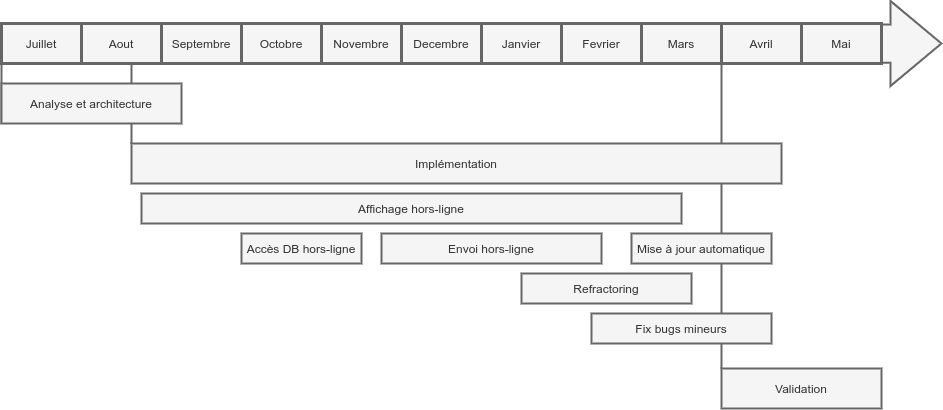
\includegraphics[width=1\textwidth]{images/Gantt}
					\caption{Diagramme de Gantt}
				\end{figure}
				
			\paragraph*{Analyse}
			Sur le schéma \ref{fig:Gantt}, on peut voir qu'il y a d'abord une grosse phase d'analyse afin de déterminer les technologies qui seraient utilisées pour les différents fonctions à implémenter. C'est dans cette phase qu'il y a eu beaucoup de discussion avec l'étudiante venue d'Haïti. En effet, il fallait utiliser des technologies qui permettrait à l'application de continuer à évoluer plus tard lorsque celle-ci serait reprise par des acteurs Haïtiens.
				C'est donc lors de cette phase qu'il a été décidé d'utiliser les services workers (PWA) plûtot que de créer une application mobile dédiée.
			
			C'est également lors de cette phase que l'on a créé un liste globale reprennant les différentes fonctionnalités principales à implémenter et leur ordre de priorité.
			
			\paragraph*{Implémentation} 
			Cette phase compose la plus grosse partie du mémoire. C'est ici que toutes les décisions prises durant la phase d'analyse se sont mise en place. Cette phase se divise en plusieur petite phase qui représente les différentes fonctionnalités produite durant le mémoire. L'avantage de travailler seul est que cela m'a permi de bien prendre en main toute l'application et pas seulement certaines parties de celle-ci car je n'avais pas la possibilité de diviser le travail. 
			Le contre partie de cela est que lorsque des problèmes de développement se présentaient, j'étais le seul à pouvoir les résoudre car personne d'autre que moi ne travaillait sur l'application. 
			
			\paragraph*{Validation}
			La phase de validation n'intervient que tard dans le déroulement du mémoire. C'est simplement parce que la méconnaissance de la technologie à utiliser et le temps qu'a prit le déploiement de l'application sur les serveurs Haïtiens ont grandement retardé l'arrivée de cette phase. Malgrès tout j'ai quand même eu le temps nécessaire pour faire passer tous les tests de validation et prendre en compte les feedbacks afin d'améliorer la production qui avait été réalisée.			
			
			
			\paragraph*{Rédaction}
			La rédaction du mémoire n'a commencé que lorsque la plupart des fonctionnalités étaient termininées. Cela a permis de lancer la validation au plus vite afin de pouvoir prendre en compte les différents feedback et d'ainsi pour les utiliser.
			Durant la rédaction, les parties produites ont été relue par mes deux promoteurs séparéments afin d'améliorer celle-ci mais aussi par des relecteurs externes afin que le texte soit plus agréable à lire. 
			
			

	\chapter{Analyse des besoins}
		\label{sec:analyse_besoins}

		% Phase essentiele blabla
		% Retouver les schémas créé début d'année

		\section{Besoins fonctionnels}

			
			%éfinition

			\subsection*{Gestion des données}
				\label{sec:gest_donnee}



			\subsection*{Affichage et accès}

			

		\section{Besoins non-fonctionnels}

			%Définition

			\subsection*{Sécurité des données}


			\subsection*{Multi-plateforme}
				

			\subsection*{Technologies simples et populaires}


		\section{Structure modulaire}
			\label{sec:modules}

			%Expliquer que mon travail conserve la structure modulaire
			%Fin du module offline
			%Lien vers ancien mémoire
			%Ajout du module "A modifier"

			

		\section{Structure des données hors-ligne}
			\label{sec:data}

			%Expliquer la différence entre données online/offline
			%Introduire ma solution

	\chapter{Implémentation}

		\section{Description de l'app de base}
			%Expliquer l'implémentation de l'app existante
				%Django
				%PostGres
				%...
		
		\section{Choix technologiques}
			\label{sec:choix_tech}
			
			\subsection*{Progressive Web-App}
				%Expliquer les différentes types d'application hors-ligne étudiée
				
			\subsection{Stratégie de synchronisation des pages}			
			
			\subsection{Stratégie de synchronisation de la DB}
			
			
			\subsection{Gestion des changements d'utilisateurs}		
			
			
			\subsection{Sytème de notification}	
						

			\subsection*{Service-worker}

		
			\subsection*{IndexedDB}

					

			\subsection*{Dexie.js}
				

			\subsection*{DataTables}

			

			\subsection*{Chart.JS}
				
				

		\section{La hiérarchie dans l'application}
			%Epliquer qu'il y a eu ou pas des changements dans le fonctionnement de l'application au niveau des modules et de la hiérachie


			\subsection*{Structure}

			

			\subsection*{Permissions}

			

		\section{Interface utilisateur}
			%Expliquer les changements faits par rapport à l'interface de base
			%Ajout de couleurs, notifications, données non-sync, ...

		\section{Client}

			%Introduction

			\subsection*{Mise en cache}
				\label{sec:cache_client}

			
			\subsection*{Gestion des données}
				Gabarits, modularité et réactivité

			\subsection*{Push des données hors-ligne}
				\label{sec:service_worker}
				
				

			

		\section{Serveur}
			\label{sec:serveur}

		

			\subsection*{Requêtes}

			

			\subsection*{Détails des requêtes API}
				\label{sec:api}

			

	\chapter{Validation}

		%Introduction

		\section{Vérifications automatiques}

			\subsection*{Tests unitaires}

			

		\section{Vérifications utilisateurs réels}


			\subsection*{Méthodologie}

				

			\subsection*{Résultats obtenus}

				

			\subsection*{Modifications apportées}

		

	\chapter{Améliorations futures}


		\section{Suite du projet}
			\label{ref:suite_projet}

		

		\section{Défis rencontrés}

			

		\section{Propositions}

			
	\chapter{Conclusion}

		

		\section{Métriques}
		

	\chapter{Bibliographie}

		\bibliographystyle{plain}
		\bibliography{bibliography.bib}
		

	

	\setlength{\parskip}{0em}
	\backcoverpage

\end{document}
